\section{A coupled, robust test norm}

In the course of our numerical experiments, we encountered unforeseen difficulties for certain problems under our current robust test norm.  We illustrate in this section the observed issue using a second model problem with a singular solution, offer possible explanations for the phenomena observed, and propose a modification of the robust test norm presented previously, which we demonstrate eliminates the issues observed in numerical experiments.  

\subsection{A second model problem}
\seclab{sec:confusionPlate}
We begin by first examining a different problem than convection-diffusion -- we examine admissible solutions for the homogeneous Laplace's equation over the $y > 0$ half-plane under boundary conditions 
\begin{align*}
u &= 0 \text{ on } x > 0\\
\pd{u}{n} &= 0 \text{ on } x < 0.
\end{align*}
Let us consider the 2D case - a simple separation of variables argument in polar coordinates shows that the solution is of the form
\[
u(r,\theta) = \sum_{n=0}^\infty R_n(r) \sin(\lambda_n \theta),
\]
where $\lambda_n = n + \frac{1}{2}$, and $R_n(r) = C_{1,n}x^{\lambda_n} + C_{2,n}x^{-\lambda_n}$.  By requiring $u(0,\theta) < \infty$, we have $R_n(r) = C_n x^{\lambda_n}$.  We have now that solutions to this problem include $u$ of the form
\[
u = \sum_{n=0} x^{n+\frac{1}{2}} \sin\LRp{\LRp{n+\frac{1}{2}}\theta}.
\]
Note that, for the lowest-order term, the gradient of $u$ displays a singularity at $r = 0$.  It is well known that, for smooth boundary data, solutions to Laplace's equation can be decomposed into the linear combination of smooth and singular contributions; the above analysis implies that, when boundary conditions change from Dirichlet to Neumann on the half-plane, the Laplace's equation will always develop a singularity in the stresses.  

Consider now Laplace's equation $\del u = f$ on the box domain $\Omega = [0,1]^2$ with boundary conditions
\begin{align*}
u &= 0 \text{ on } x > .5\\
\pd{u}{n} &= 0 \text{ on } x < .5.
\end{align*}
with forcing term $f=1$.  
\begin{figure}[!h]
\centering
\subfigure{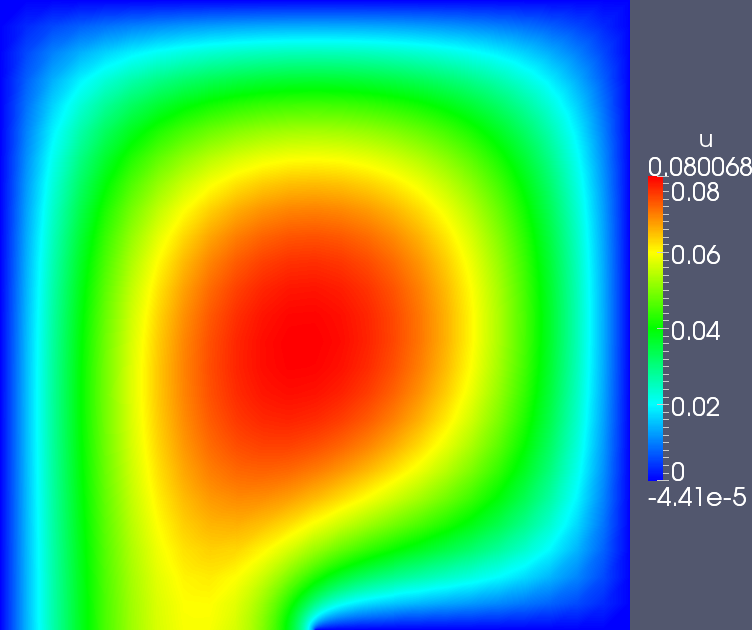
\includegraphics[scale=.375]{figs/LaplaceFigs/LaplacePlate.png}}
\caption{Solution of Laplace's equation on the unit quad with $f=1$.}
\label{fig:laplace}
\end{figure}
Extrapolating the results from the half-plane example to a finite domain, we expect the solution of Laplace's equation to be bounded, but to have a singularity in its gradient.  Figures~\ref{fig:laplace} and \ref{fig:laplaceStresses} are finite element solutions of the above problem under a quadratic $h$-refined mesh.  Figure~\ref{fig:laplace} confirms that $u$ is bounded, while Figure~\ref{fig:laplaceStresses} confirms that singularities in the gradient appear at the point $(.5,0)$, where the boundary condition changes from Neumann to Dirichlet.  

\begin{figure}[!h]
\centering
\subfigure{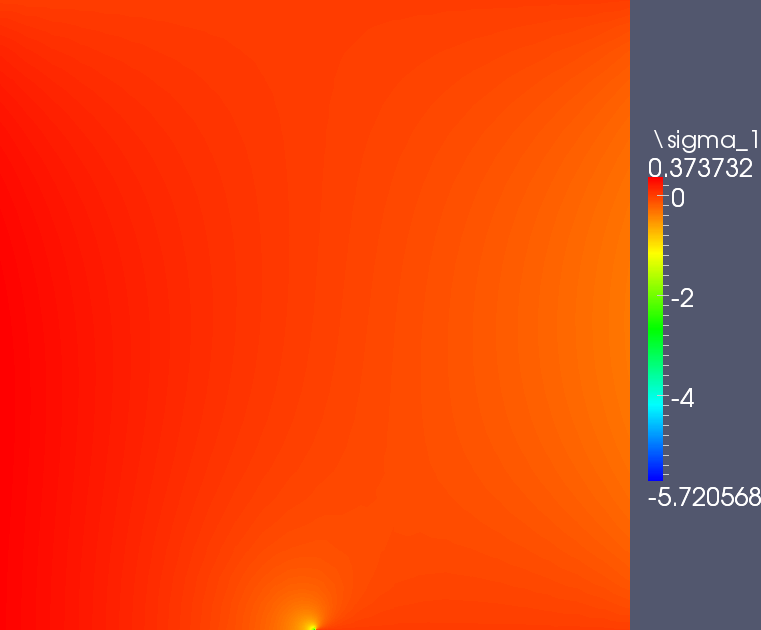
\includegraphics[scale=.275]{figs/LaplaceFigs/LaplacePlateSigma1.png}}
\subfigure{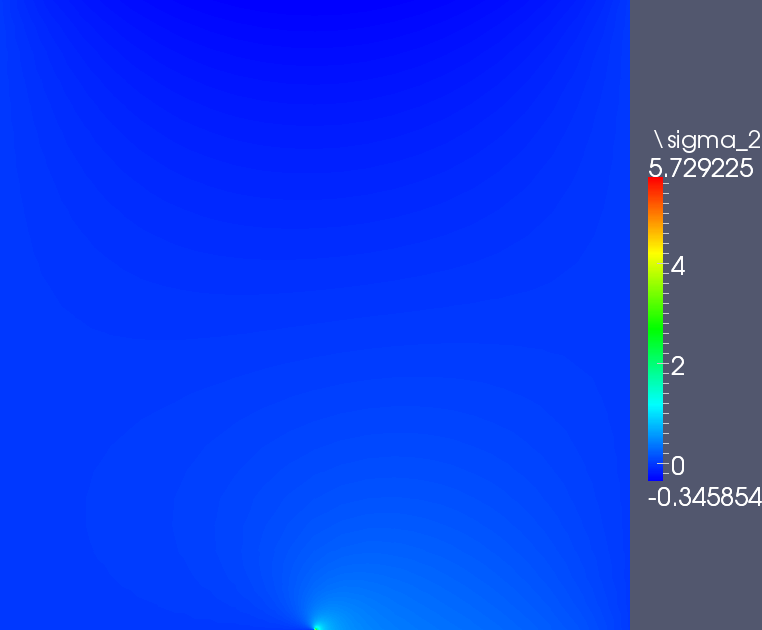
\includegraphics[scale=.275]{figs/LaplaceFigs/LaplacePlateSigma2.png}}
\caption{$x$ and $y$ components of the $\Grad u$ for $u$ solving Laplace's equation with a change in boundary conditions.  Both components develop singularities at the point where the boundary condition changes type.}
\label{fig:laplaceStresses}
\end{figure}

We consider now the convection-diffusion problem, under a similar setup as before.  We consider the domain $\Omega = [0,1]^2$, with boundary conditions
\begin{align*}
u &= 0,\quad \text{ on } x = 0\\
\pd{u}{n} &= 0,\quad \text{ on } x = 1, y = 1, \text{ and } y = 0, x < .5\\
u &= 1,\quad \text{ on } .5 < x \leq 1.
\end{align*}
The problem is meant to simulate the transport of $u$ over a domain with a ``plate'' boundary $x \in [.5,1]$.  For small $\epsilon$, the problem develops a boundary layer over the plate, as well as a singularity at the plate tip $(x,y) = (.5,0)$.\footnote{This problem is meant to mimic the Carter flat plate problem -- a common early benchmark problem in viscous compressible flow problems -- which can be shown to also exhibit a singularity in stress at the point $(.5,0)$.}  Unlike the Laplace example, we swap the Dirichlet boundary condition at the outflow $x=1$ with an outflow boundary condition.\footnote{The outflow ``boundary condition'' is simply the absence of an applied boundary condition, and is analyzed in more detail in \cite{FLD:FLD505}.  This outflow condition appears to work well for convection-diffusion problems in the convective regime, and is the outflow condition we will use in our extension of DPG to a model problem in viscous compressible flow.  Though the well-posedness of the problem under this boundary condition is questionable, we can still effectively illustrate the issues present under the robust test norm using this problem setup.  }

The above convection-diffusion problem is related back to the earlier Laplace/diffusion problem with a singularity -- in most of the domain, convective effects dominate; however, if we  localize the behavior of Laplace's equation to a circle of $\epsilon$ around $(.5,0)$, then we again see a discontinuity in the stresses.  Asymptotic expansion techniques indicate that singularities in solutions are determined primarily by the highest order differential operator present in the equation -- in other words, the addition of a convective term to a scaled Laplacian (to recover the convection-diffusion equation) will not alter the presence of a singularity in the solution.  

\begin{figure}[!h]
\centering
\subfigure{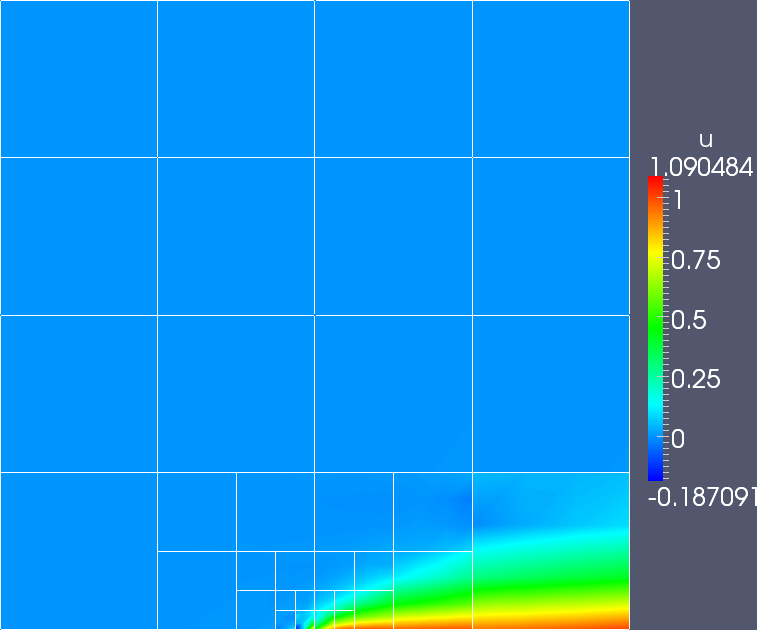
\includegraphics[scale=.275]{figs/LaplaceFigs/confusion1e2h1e2.png}}
\subfigure{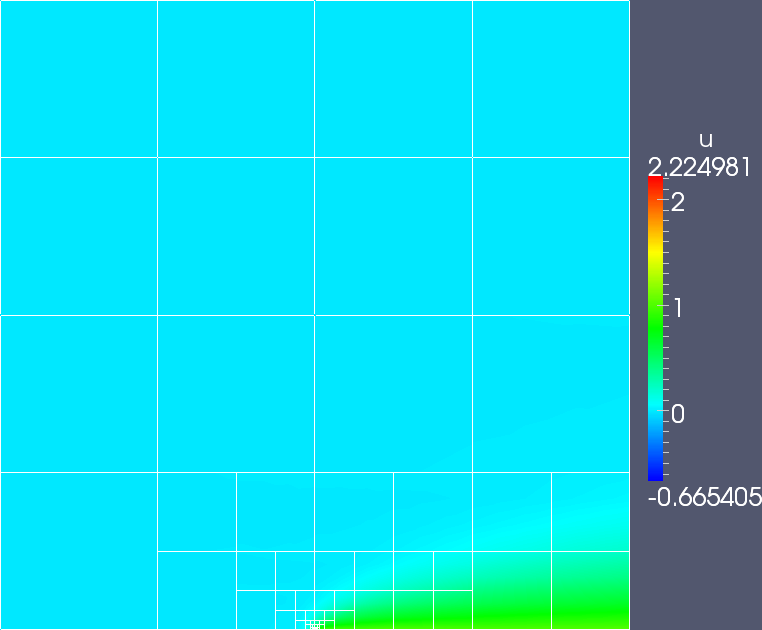
\includegraphics[scale=.275]{figs/LaplaceFigs/confusion1e2h1e3.png}}
\caption{Solution $u$ for $\epsilon = .01$ under the robust test norm.  The solution oscillates strongly at the plate edge, growing in magnitude under additional refinements despite the absence of a singularity in $u$ at that point.}
\label{fig:plateOsc}
\end{figure}

Figures~\ref{fig:plateOsc} and \ref{fig:plateOscZoom} demonstrate the behavior of the DPG method under the robust test norm for the plate problem.  The diffusion is taken to be fairly large ($\epsilon = 10^{-2}$), and automatic refinements are done until the element size $h$ is at or below the diffusion scale.  Due to the singular nature of the solution, refinements are clustered around $(.5,0)$, and the order is set to be uniform with $p=2$.  While there should be no singularity in $u$, the magnitude of $u$ grows as $h \rightarrow 0$, so long as $h\leq \epsilon$.  

\begin{figure}[!h]
\centering
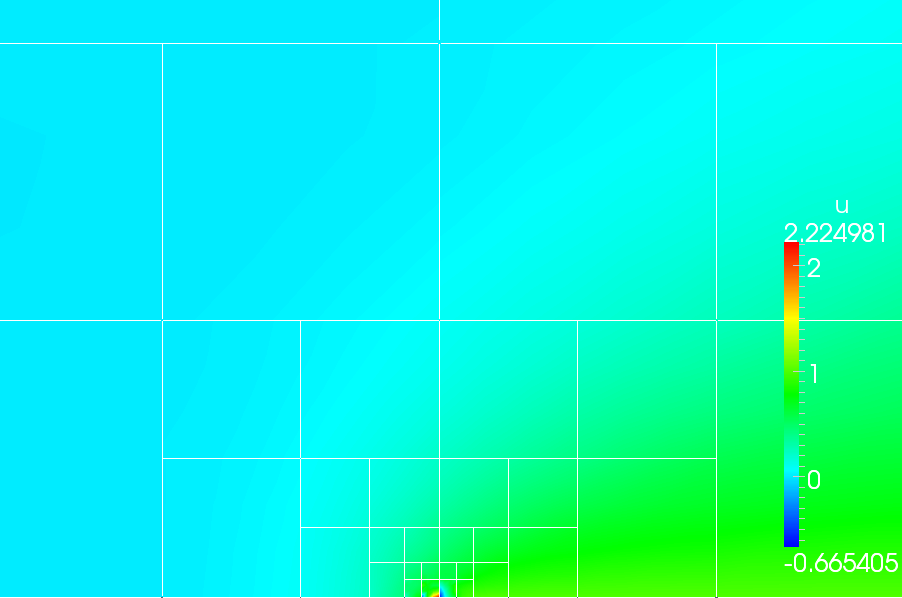
\includegraphics[scale=.375]{figs/LaplaceFigs/confusion1e2h1e3uZoom.png}
\caption{Zoomed solution $u$ and adaptive mesh for $\epsilon = .01$ after over-resolution of the diffusion scale. }
\label{fig:plateOscZoom}
\end{figure}

We note that the appearance of this non-physical singularity in $u$ is allowed under the theory underlying the robust test norm; the error in the $\L$-norm of the solution is guaranteed to be robustly bounded; however, the $\L$ norm does allow for the presence of weak singularities (singularities of order $x^{-\frac{1}{2}}$).  Apart from the oscillation of $u$ at the singular point, the solution is well-behaved, and the stress $\sigma = \epsilon \Grad u$ is very well represented, as indicated in Figure~\ref{fig:plateStresses}.  

\begin{figure}[!h]
\centering
\subfigure{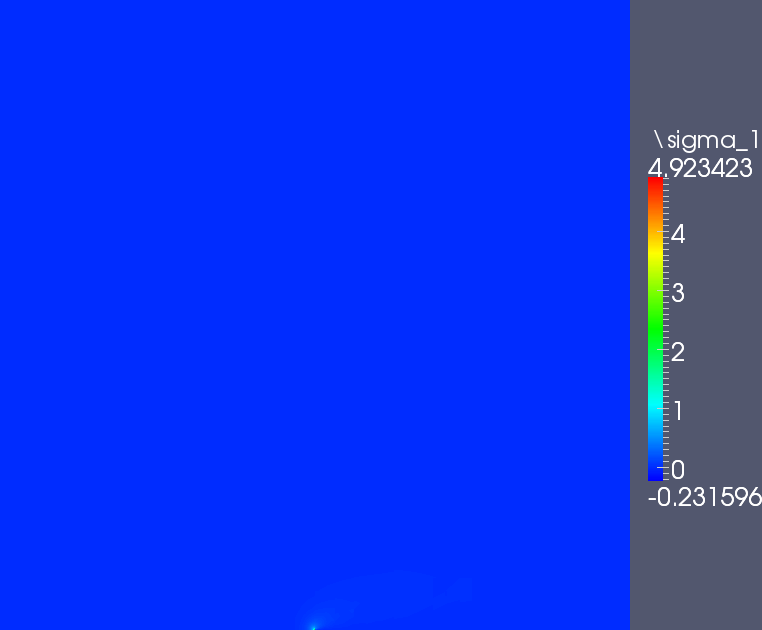
\includegraphics[scale=.275]{figs/LaplaceFigs/confusion1e2h1e3Sigma1.png}}
\subfigure{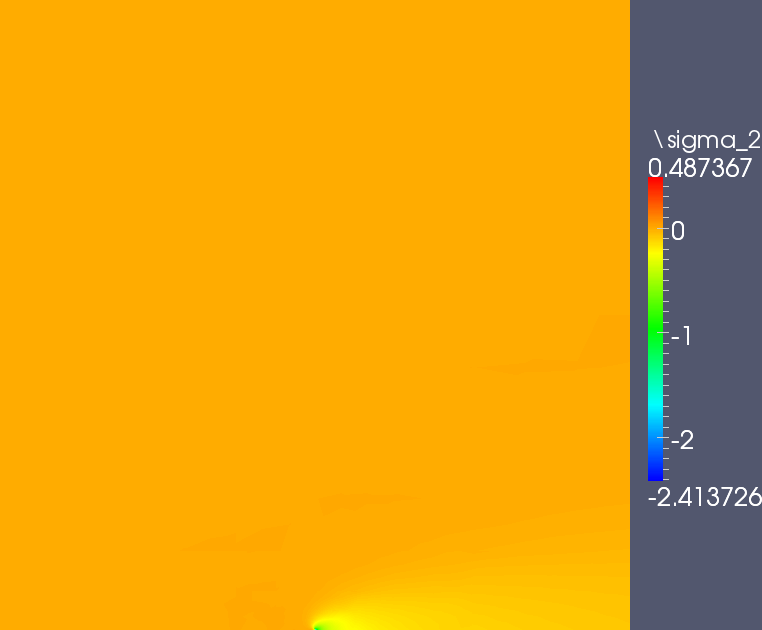
\includegraphics[scale=.275]{figs/LaplaceFigs/confusion1e2h1e3Sigma2.png}}
\caption{Viscous stresses for the plate problem.  }
\label{fig:plateStresses}
\end{figure}

\subsection{A modification of the robust test norm}

While oscillations of this sort in a solution near a singular point may be acceptable in certain simulations, it is a large problem for the methods in compressible flow simulations -- physical constraints require several solution variables to remain positive throughout simulation.\footnote{Apart from returning a non-physical solution, the violation of positivity constraints typically results in non-convergence of nonlinear solvers.}  We propose a modification of the robust test norm that appears to remedy this issue, which we refer to as 
\[
\nor{\LRp{v,\tau}}_V^2 \coloneqq \nor{v}^2_{\L} + \epsilon \nor{\grad v}^2_{\L} + \nor{\beta\cdot \Grad v}_{\L}^2 + \nor{\div \tau - \beta\cdot\Grad v}_{\L}^2 + \nor{C_\tau\tau}_{\L}^2,
\]
where $C_\tau$ is defined as before.\footnote{We note that we have dropped the mesh-dependent scaling on $\nor{v}_{\L}$ from the robust norm; this is related to recent insights into the nature of DPG test spaces and explained in more detail in Appendix~\secref{appendix:globalLocal}.}  We note that, under the theory developed in Section~\secref{sec:testNormSec}, the above test norm is trivially provably robust using the same theory.\footnote{This is due to the fact that $\nor{\div \tau - \beta\cdot\Grad v}_{\L}^2$ is robustly bounded by $\nor{\div \tau}_{\L}$ and $\nor{\beta\cdot\Grad v}_{\L}$.  Alternatively, we can note that $\nor{\div \tau - \beta\cdot\Grad v}_{\L}^2 = \nor{g}_{\L}^2$, where $g$ is a load of the adjoint problem related to robustness described in Section~\secref{sec:testNormSec}.}

While not rigorously understood, the author believes the issues related to the appearance of non-physical singularities to be related to the uncoupled nature of the test norm.  Previous example problems exhibited boundary layers and sharp gradients in the stress $\sigma$, but not singularities, which contribute significantly more error.  We expect that the oscillations observed in $u$ are a sort of \textit{pollution error}, where error in $u$ is tied to error in $\sigma$.  If we consider the ultra-weak variational formulation for convection-diffusion
\[
\LRp{u,\div \tau - \beta\cdot \grad v}_{\L} + \LRp{\sigma,\frac{1}{\epsilon} \tau + \grad v}_{\L} + \ldots,
\]
we can see that it is a combination of test functions that corresponds to both $u$ and $\sigma$.  Recall from the previous section that, by choosing $\tau$ and $v$ such that they satisfy the adjoint equation with forcing terms $u$ and $\sigma$, we recover the best $L^2$ approximation.  In other words, achieving optimality in the $L^2$ norm requires coupling between $v$ and $\tau$, which is achieved under the graph norm, but not the robust norm derived in the previous section.  If coupling of the test terms delivers optimality in $u$ and $\sigma$ independently, we expect that decoupling $v$ and $\tau$ from each other in a test norm from each other will have the effect of coupling error in $\sigma$ to error in $u$, which would explain the spurious oscillations in $u$ in the presence of singularities in $\sigma$.\footnote{Similar results have been observed in the Stokes equations, where error in $u$ is coupled to the behavior of the pressure variable \cite{FLD:FLD582}.} 

The drawback to using the above test norm is that the resulting local system for test functions is now completely coupled, whereas using the previous test norm, the system was block diagonal due to the decoupling in $v$ and $\tau$ and could be constructed and inverted more efficiently.  We hope to explore the difference between these two norms in more rigor and detail in the future; however, experiments in \cite{localConservationDPG} indicate that this new norm performs equivalently or better than the robust test norm derived in the previous chapter for a large range of numerical examples.

\begin{figure}[!h]
\centering
\subfigure{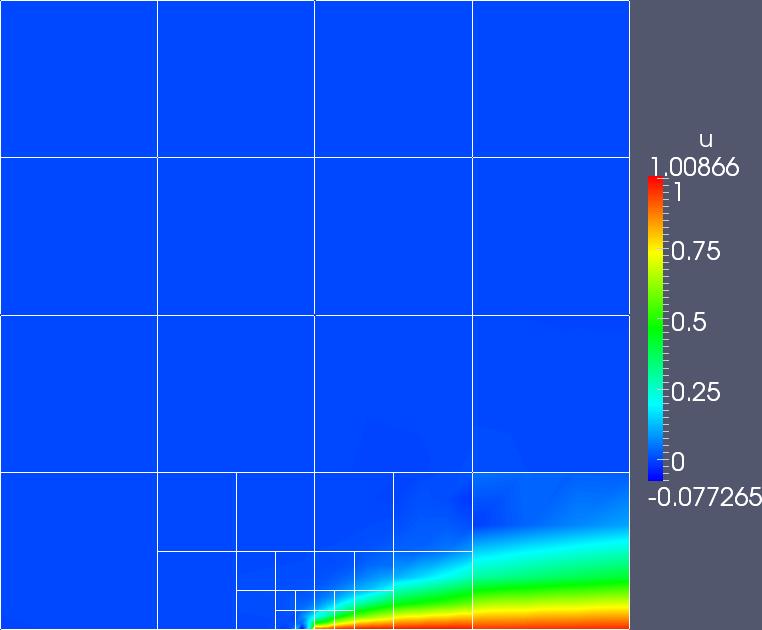
\includegraphics[scale=.275]{figs/LaplaceFigs/coupled1e2h1e2.png}}
\subfigure{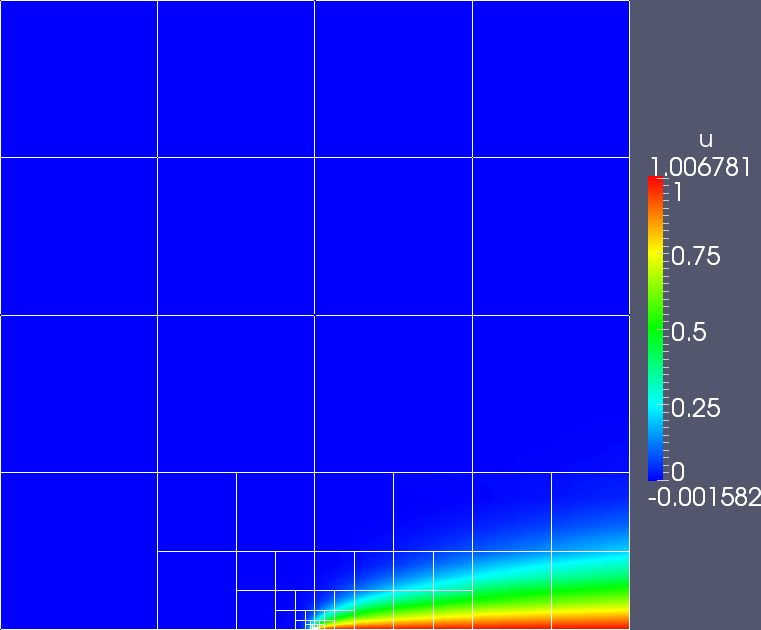
\includegraphics[scale=.275]{figs/LaplaceFigs/coupled1e2h1e3.png}}
\caption{$\epsilon = 10^{-2}$ without $h$-resolving diffusion scale, and with $h$-resolution of diffusion scale.}
\label{fig:newNorm}
\end{figure}

Figure~\ref{fig:newNorm} shows the solution for $\epsilon = .01$, where the diffusion scale is both underresolved and resolved by $h$-adaptivity.  In both cases, there are no additional oscillations near the plate tip -- Figure~\ref{fig:newNormZoom} shows a zoomed image of the solution $u$ at the point $(.5,0)$.  The stress is resolved similarly to the previous case; however, the solution $u$ does not display spurious oscillations in either the underresolved or resolved cases.  Figure~\ref{fig:newNormSmallEps} displays the same quantities, but for $\epsilon = 10^{-4}$, in order to demonstrate that the new test norm removes spurious oscillations in $u$ (in the presence of singularities in $\sigma$) independently of $\epsilon$.  

\begin{figure}[!h]
\centering
%\subfigure{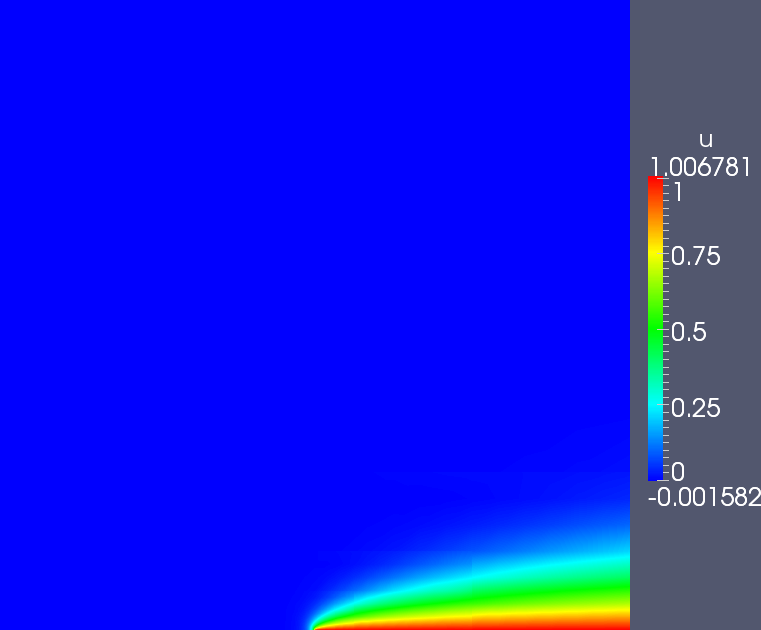
\includegraphics[scale=.25]{figs/LaplaceFigs/coupled1e2h1e3u.png}}
%\subfigure{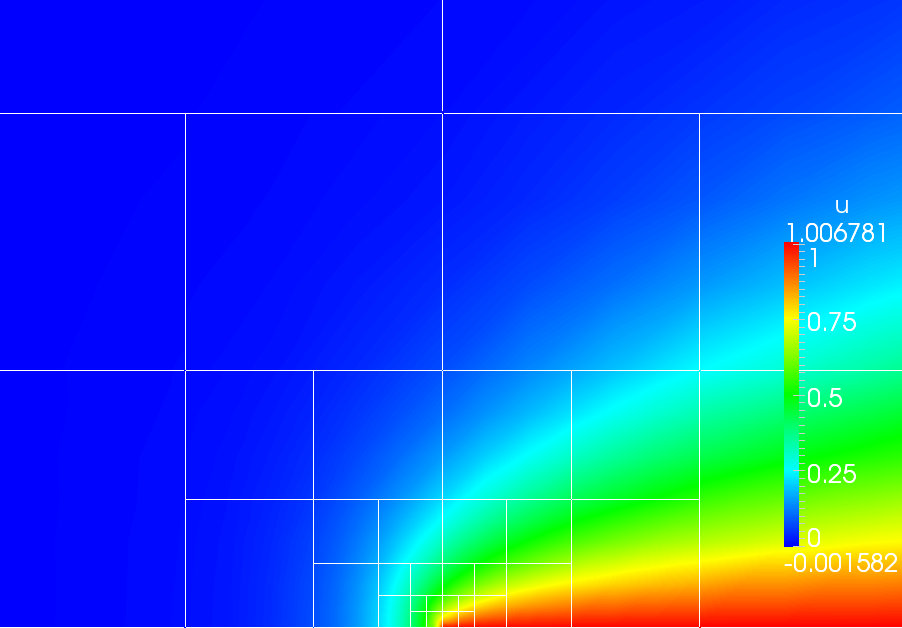
\includegraphics[scale=.251]{figs/LaplaceFigs/coupled1e2h1e3uZoom.png}}
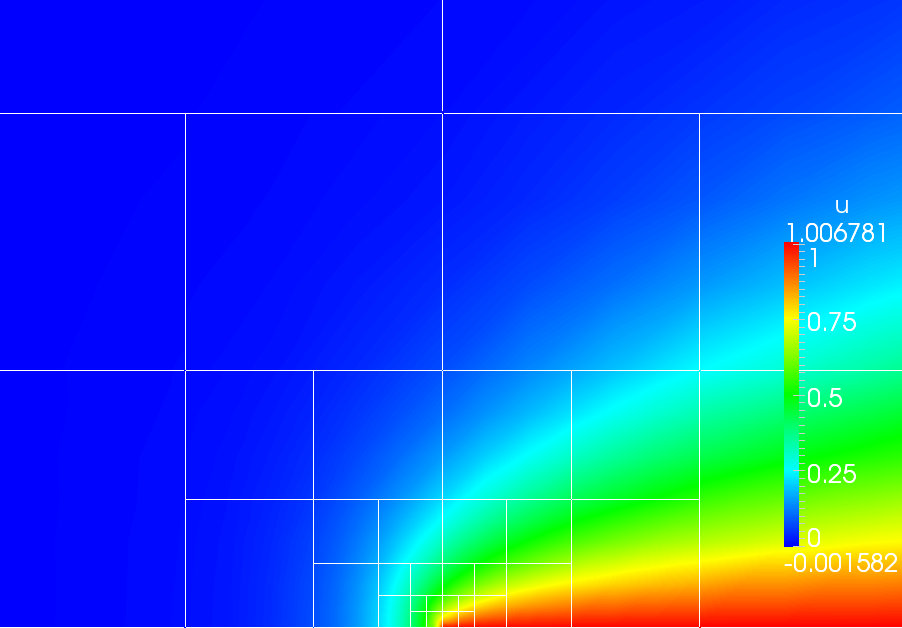
\includegraphics[scale=.3]{figs/LaplaceFigs/coupled1e2h1e3uZoom.png}
\caption{Zoom of solution $u$ at the plate tip for $\epsilon = 10^{-2}$.}
\label{fig:newNormZoom}
\end{figure}

\begin{figure}[!h]
\centering
\subfigure{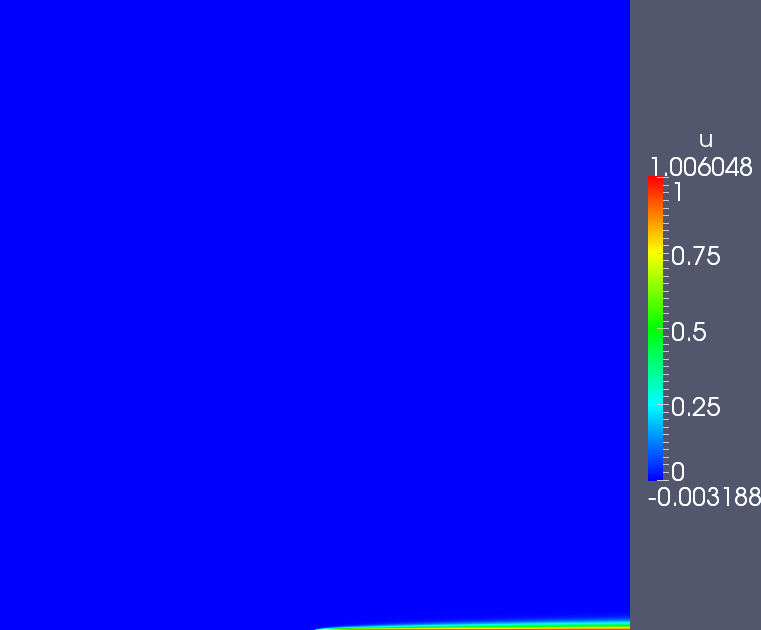
\includegraphics[scale=.25]{figs/LaplaceFigs/coupled1e4h1e5.png}}
\subfigure{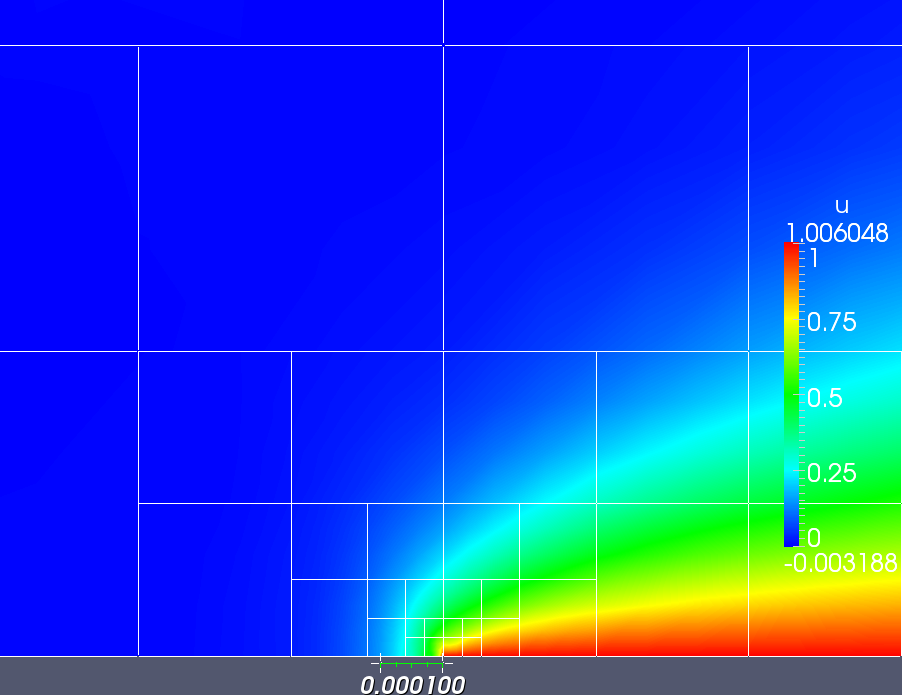
\includegraphics[scale=.227]{figs/LaplaceFigs/coupled1e4h1e5Zoom.png}}
\caption{14 refinements for $\epsilon = 10^{-4}$, min $h$ is $O(10^{-5})$.}
\label{fig:newNormSmallEps}
\end{figure}

\section{Anisotropic refinement}
\seclab{sec:aniso}
Isotropic adaptive mesh refinement has shown itself to be an effective way to resolve isolated solution features with large gradients, such as point singularities \cite{hp1,hp3}. However, for the resolution of phenomena such as shocks or boundary layers, anisotropic mesh refinement can resolve solution features for a much lower cost per degree-of-freedom, due to the fact that boundary layers in $n$-dimensions are primarily phenomena supported over $n-1$ dimensions.  

As a least squares method, DPG already includes a natural error indicator with which to drive adaptive mesh refinement.  To introduce anisotropic refinements, we need to introduce an anisotropy indicator in order to detect in which direction solution features are aligned.  In general, a test norm can be expressed as the sum of normed quantities, both scalar and vector valued.  If we restrict ourselves to quadrilateral elements for the moment, a general anisotropy indicator for DPG can be constructed by evaluating the $\L$ norms of the individual components of vector valued terms in the test norm.  

Under the robust test norm derived in this chapter for the convection-dominated diffusion problem, we can define $x$ and $y$ error contributions over a single element
\begin{align*}
e_{x,K} &= \epsilon \nor{\pd{v}{x}}_{L^2(K)}^2 + \nor{\tau_x}_{L^2(K)}^2 \\
e_{y,K} &= \epsilon \nor{\pd{v}{y}}_{L^2(K)}^2 + \nor{\tau_y}_{L^2(K)}^2.
\end{align*}
We define the anisotropy indicator as the ratio $r_K = \frac{e_{x,K}}{e_{y,K}}$, and implement a simple refinement scheme following \cite{DPG3}.  Given some anisotropic threshold $\epsilon_r$, if $r_K>\epsilon_r$, then we can conclude that the error in the $x$ direction is large compared to the $y$ direction, and we anisotropically refine the element along the $x$-axis.  Likewise, if $r_K < \frac{1}{\epsilon_r}$, this implies that the opposite is true, and we refine the element anisotropically along the $y$-axis.  

We note that it is possible to compute the discrete system without needing much additional integration.  Recall that if we let $G$ be the symmetric positive-definite Gram matrix representing the inner product $\LRp{v,\delta v}_V$ on $V_h$, we solve for degrees of freedom $c_e$ representing our error representation function $e$.  

For both the graph and robust test norms, we can decompose the inner product that induces the test norm into 
\[
\LRp{v,\delta v}_V = \sum_i \LRp{v,\delta v}_{V,x_i} + \LRp{v,\delta v}_{V,{\rm scalar}}
\]
such that $\LRp{v,\delta v}_{V,x_i}$ is a seminorm containing the $i$th coordinate component of a vector-valued test term, and $\LRp{v,\delta v}_{V,{\rm scalar}}$ is simply the non-vector portions of the test norm.  For example, if we take the $H^1(\Omega)$ Sobolev norm
\[
\LRp{v,\delta v}_V = \LRp{v,\delta v}_{\L} + \LRp{\grad v,\grad \delta v}_{\L}
\]
then $\LRp{v,\delta v}_{V,x_i} = \LRp{\pd{v}{x_i},\pd{\delta v}{x_i}}_{\L}$, and $\LRp{v,\delta v}_{V,{\rm scalar}} = \LRp{v,\delta v}_{\L}$.  Each bilinear term $\LRp{v,\delta v}_{V,x_i}$ induces a symmetric positive-semidefinite matrix $G_{x_i}$, such that 
\[
c_e^TG_{x_i}c_e = \nor{e}^2_{V,x_i}.
\]
By storing $G$ as the sum of $G_{\rm scalar}$ and $G_{x_i}$, we can then cheaply compute the anisotropic error indicators once we have the degrees of freedom corresponding to our error representation function.  

%\textcolor{red}{Add examples of anisotropic refinement for plate/boundary layers}

